% Aidan Hunt
% 4/21/2023

% Additional output cases

% Packages for presenting code
\documentclass{article}
\usepackage{listings}
\usepackage{pythonhighlight}
\usepackage{graphicx}

\begin{document}

\section*{Output Example 1}

\begin{python}
### Main body of the script ### 
# Define properties of several airfoils
profileNames = ['NACA0018', 'naca 0025', 'NACA0008']
chords = [4, 6, 7]
angles = [0, 45, -30]

# Call function to compute coordinates and plot airfoils
foilCoords = computeAirfoils(profileNames, chords, angles)
\end{python}

\begin{figure}[h]
    \centering
    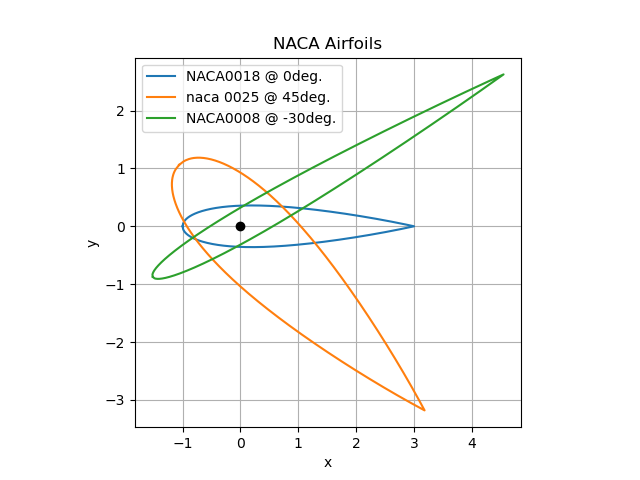
\includegraphics[width=\textwidth]{exOutput.png}
\end{figure}

\newpage

\section*{Output Example 2}

\begin{python}
    profileNames = ['NACA0018', 'NACA0018', 'NACA0018', 
                    'NACA0018', 'NACA0018', 'NACA0018']
    chords = [1, 2, 3, 4, 5, 6]
    angles = [0, 10, 20, 30, 40, 50]
    
    foilCoords = computeAirfoils(profileNames, chords, angles)
\end{python}

\begin{figure}[h]
    \centering
    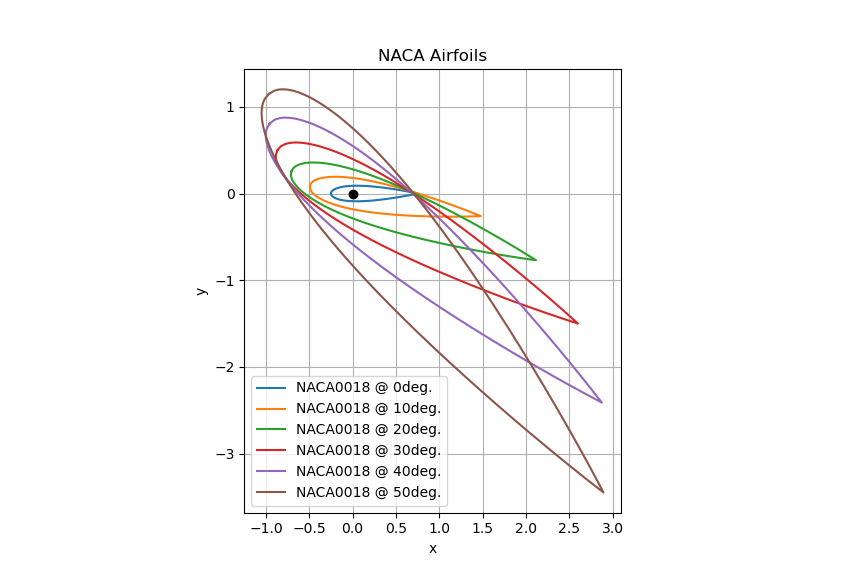
\includegraphics[width=\textwidth]{exOutput2.png}
\end{figure}

\newpage

\section*{Output Example 3}

\begin{python}
    profileNames = 'nAcA      0018'
    chords = 4.06
    angles = 6
    foilCoords = computeAirfoils(profileNames, chords, angles)
\end{python}

\begin{figure}[h]
    \centering
    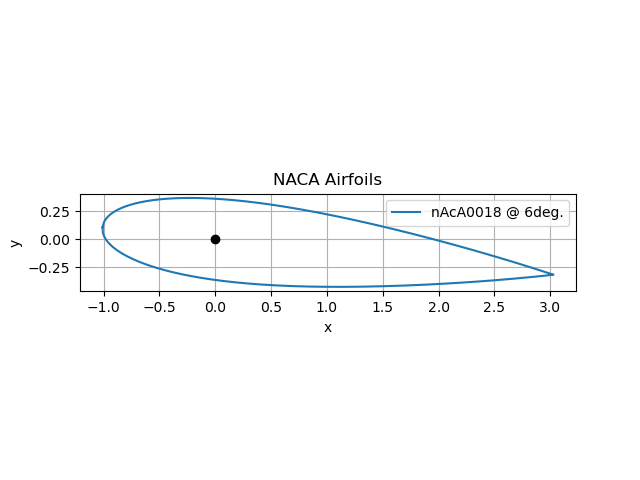
\includegraphics[width=\textwidth]{exOutput3.png}
\end{figure}

\end{document}